\documentclass[11pt]{article}
\usepackage[letterpaper,margin=1in]{geometry}
\usepackage{microtype}   % better justification at the wider measure
\usepackage[utf8]{inputenc}
\usepackage{amsmath}
\usepackage{graphicx}
\usepackage[numbers,sort&compress]{natbib}
\usepackage{booktabs}
\usepackage{xcolor}
\usepackage{hyperref}
\definecolor{linknavy}{RGB}{0,70,140}
\hypersetup{
  colorlinks = true,
  citecolor  = linknavy,   % [1] citation numbers -> jump to the bibliography
  linkcolor  = linknavy,   % \ref / \S cross-references
  urlcolor   = linknavy,   % \url and bibliography links
  breaklinks = true,
}
\usepackage{parskip}
\usepackage{tikz}
\usetikzlibrary{arrows.meta, positioning, calc}

% --- Short-form reference in the page footer at every citation -------------
% \citetf / \citepf behave exactly like \citet / \citep, and additionally drop
% a short-form note into the footer of the page where the citation occurs:
%     [6] Socher et al. (2013), Recursive Deep Models..., EMNLP.
% Author and year are pulled from the .bib via natbib (no duplicated data);
% the leading [n] links to the full entry in the bibliography, which carries
% the complete details and the URL. Multi-key cites emit one note per key.
\makeatletter
% Per-key short title + venue. This is the only hand-maintained data; keep the
% key set in sync with references.bib.
\newcommand{\shortref}[2]{\expandafter\gdef\csname sr@#1\endcsname{#2}}
\shortref{socher2013sst}      {Recursive Deep Models over a Sentiment Treebank, EMNLP}
\shortref{wang2019glue}       {GLUE: A Multi-Task Benchmark for NLU, ICLR}
\shortref{hendrycks2021mmlu}  {Measuring Massive Multitask Language Understanding, ICLR}
\shortref{williams2018mnli}   {A Broad-Coverage Challenge Corpus for Sentence Understanding through Inference, NAACL}
\shortref{mcnemar1947note}    {Sampling Error of the Difference Between Correlated Proportions, Psychometrika}
\shortref{edwards1948note}    {Correction for Continuity in Correlated Proportions, Psychometrika}
\shortref{efron1993bootstrap} {An Introduction to the Bootstrap, Chapman \& Hall}
\shortref{koehn2004significance}{Statistical Significance Tests for MT Evaluation, EMNLP}
\shortref{sporleder2009idiom} {Literal and Non-Literal Use of Idiomatic Expressions, EACL}
\shortref{tayyar2021astitch}  {AStitchInLanguageModels: Idiomaticity in Pre-Trained LMs, Findings of EMNLP}
\shortref{chakrabarty2022flute}{FLUTE: Figurative Language Understanding through Textual Explanations, EMNLP}
\shortref{jia2017adversarial} {Adversarial Examples for Evaluating Reading Comprehension, EMNLP}
\shortref{ribeiro2018semantically}{Semantically Equivalent Adversarial Rules for Debugging NLP Models, ACL}
% Falls back to the bare citation if a key has no short form registered.
\newcommand{\fn@short}[1]{%
  \footnote{\citep{#1} \citeauthor{#1} (\citeyear{#1})%
    \@ifundefined{sr@#1}{}{, \csname sr@#1\endcsname}.}}
\newif\iffn@first
% comma between consecutive markers, so a two-key cite reads "11,12" not "1112"
\newcommand{\fn@sep}{\iffn@first\fn@firstfalse\else\textsuperscript{,}\fi}
\newcommand{\footeach}[1]{%
  \fn@firsttrue
  \@for\@fnkey:=#1\do{\fn@sep\expandafter\fn@short\expandafter{\@fnkey}}}
\makeatother
\newcommand{\citetf}[1]{\citet{#1}\footeach{#1}}
\newcommand{\citepf}[1]{\citep{#1}\footeach{#1}}

\title{Does Idiomatic Phrasing Degrade LLM Task Performance? \\
A Controlled Paraphrase-vs-Idiom Study Across Instruction-Tuned Decoder Models}
\author{Student name (ID. XXXXXXXXX)} % TODO: fill in name(s) / ID(s)
\date{Submitted as final project report for the NLP course, Reichman University, 2026}

\begin{document}

\maketitle

\section{Introduction}

It is a widely held assumption in NLP that idiomatic language (expressions
whose meaning cannot be derived compositionally from their individual words,
e.g. \emph{``spill the beans''} or \emph{``par for the course''}) is
harder for language models to understand than direct, literal phrasing.
Idioms are non-compositional, culturally specific, and comparatively rare in
naturally-occurring balanced training data relative to literal phrasing of
the same content, so this assumption is intuitive. However, it is rarely
tested \emph{in isolation}: any two rewordings of the same sentence already
differ from each other lexically and syntactically, so a naively observed
accuracy drop after ``idiomatizing'' a sentence could simply be an artifact
of rewording in general, rather than something specific to idiomaticity.

\textbf{Central research question:} does phrasing a task input
idiomatically cause a measurable degradation in a language model's task
accuracy, \emph{over and above} the degradation that any comparable
paraphrase (a non-idiomatic rewording) already causes?

To answer this cleanly, every original example $x$ in this project is
rewritten into two controlled variants that share the same rewriting budget
but differ in exactly one property:

\begin{itemize}
  \item $x_{\text{paraphrase}}$: reworded in different words,
    \textbf{without} idioms. This is the \emph{control} condition; it
    isolates the effect of rewording/rephrasing alone.
  \item $x_{\text{idiomatic}}$: reworded \textbf{with} one or more natural
    idiomatic expressions, preserving the same meaning.
\end{itemize}

The task label $y$ is preserved across all three variants (original,
paraphrase, idiomatic) by construction (see \S\ref{sec:augmentation}). A
model is evaluated on all three variants with an identical prompt template,
so that only the surface form of the input text changes between runs. This
paired design lets us attribute any additional degradation seen under the
idiomatic variant, beyond what the paraphrase variant already causes, to
idiomaticity specifically rather than to rewording in general.

This question matters practically: idiomatic language is common in the kind
of user-generated text that deployed NLP systems must handle robustly, such
as product reviews, customer support transcripts, informal social media
posts, and everyday conversation. If idiomaticity has a genuine, isolable
negative effect on model accuracy, that has direct implications for prompt
engineering, data augmentation strategies, and robustness evaluation of
deployed systems. If it does not, i.e. if apparent idiom-related failures
are really just generic paraphrase sensitivity, then effort spent
specifically on idiom-handling may be misplaced relative to general
robustness-to-rewording work.

\textbf{Contributions.} This project's main contributions are:
\begin{enumerate}
  \item \textbf{A paraphrase-controlled three-way design.} Each input is
    rewritten into paired original / paraphrase / idiomatic variants, so the
    paraphrase arm absorbs the generic cost of rewording and leaves the
    idiom-specific effect isolated.
  \item \textbf{A sole-cause diagnostic.} Restricted to items a model already
    answers correctly, it identifies which single rewrite is responsible when
    exactly one of the two flips the answer, attributing degradation to a
    transformation rather than to ordinary variance.
  \item \textbf{Dual significance testing.} Every sole-cause result is tested
    with a continuity-corrected McNemar test and cross-checked against an
    independent non-parametric bootstrap, guarding against the chi-square
    approximation on small discordant-pair counts.
  \item \textbf{Breadth across models and tasks.} Eleven instruction-tuned
    decoder LLMs (roughly 0.5B--9B parameters, six model families) evaluated
    on three datasets spanning sentiment, knowledge QA, and inference, with a
    pooled cross-model test.
  \item \textbf{A reproducible four-stage pipeline} (clean $\rightarrow$
    augment $\rightarrow$ evaluate $\rightarrow$ analyze) with LLM-judge
    validation of every augmented example and per-artifact provenance
    (\S\ref{sec:methodology}).
\end{enumerate}

\subsection{Related Work}

\textbf{Idiom processing in NLP.} Prior work on idiomatic language in NLP has
mostly focused on \emph{detecting} or \emph{translating} idioms, rather than
measuring their effect on downstream task accuracy. \citetf{sporleder2009idiom}
study token-level classification of literal versus idiomatic usage of a given
expression in context. \citetf{tayyar2021astitch} probe pretrained language
models specifically on their ability to distinguish idiomatic from literal
usage, finding that such models detect idiomatic usage reasonably well when
given one or a few in-context examples of an expression, but degrade
substantially in the zero-shot setting on expressions unseen during
training. \citetf{chakrabarty2022flute} introduce a benchmark (FLUTE, 9{,}000
instances) for figurative language understanding covering idioms, similes,
metaphors, and sarcasm, framed as natural language inference with
explanation generation. These works establish
that idiom \emph{comprehension} is a genuine weak point for language models,
but do not isolate how much of an idiom's effect on a \emph{downstream task}
(e.g. sentiment classification, multiple-choice QA) is attributable to
idiomaticity itself versus the generic effect of rewording a sentence.

\textbf{Paraphrase and rewording robustness.} A separate line of work shows
that models are sensitive to paraphrasing and adversarial rewording that
preserves meaning: \citetf{jia2017adversarial} show reading-comprehension
models can be fooled by distractor sentences that do not change the correct
answer, and \citetf{ribeiro2018semantically} show semantics-preserving
rewrites (SEARs) can flip model predictions across several NLP tasks. This
motivates why a bare original-vs-idiomatic comparison is confounded: any
degradation observed could simply be this generic paraphrase-sensitivity
phenomenon, not something specific to idioms. To our knowledge, no prior
work explicitly isolates idiom-specific degradation from generic
paraphrase-induced degradation via a paired three-way control design across
a broad panel of contemporary open instruction-tuned decoder LLMs, which is
the gap this project addresses.

\textbf{Datasets and statistical methodology.} We build on three established
benchmarks: SST-2 \citepf{socher2013sst,wang2019glue}, a binary sentiment
classification dataset built from movie-review snippets; MMLU
\citepf{hendrycks2021mmlu}, a multi-domain multiple-choice knowledge
benchmark; and MultiNLI \citepf{williams2018mnli}, a three-way natural
language inference corpus of roughly 433k sentence pairs spanning ten written
and spoken genres. For
paired significance testing on per-example correctness we use
McNemar's test \citepf{mcnemar1947note} with a continuity correction
\citepf{edwards1948note}, the standard approach for paired nominal
before/after comparisons, cross-validated with paired non-parametric
bootstrap resampling \citepf{efron1993bootstrap,koehn2004significance}.

\section{Methodology}
\label{sec:methodology}

\subsection{Pipeline overview}

The project is implemented as four explicit, independently re-runnable
stages that communicate only through versioned files on disk, plus YAML
configuration files that fully determine each stage's behavior. This design
means any stage can be re-executed on its own (re-running evaluation for a
new model, for instance, does not require repeating cleaning or
augmentation), and every artifact records the configuration hash and
model/prompt version that produced it, for full provenance.

\begin{figure}[t]
\centering
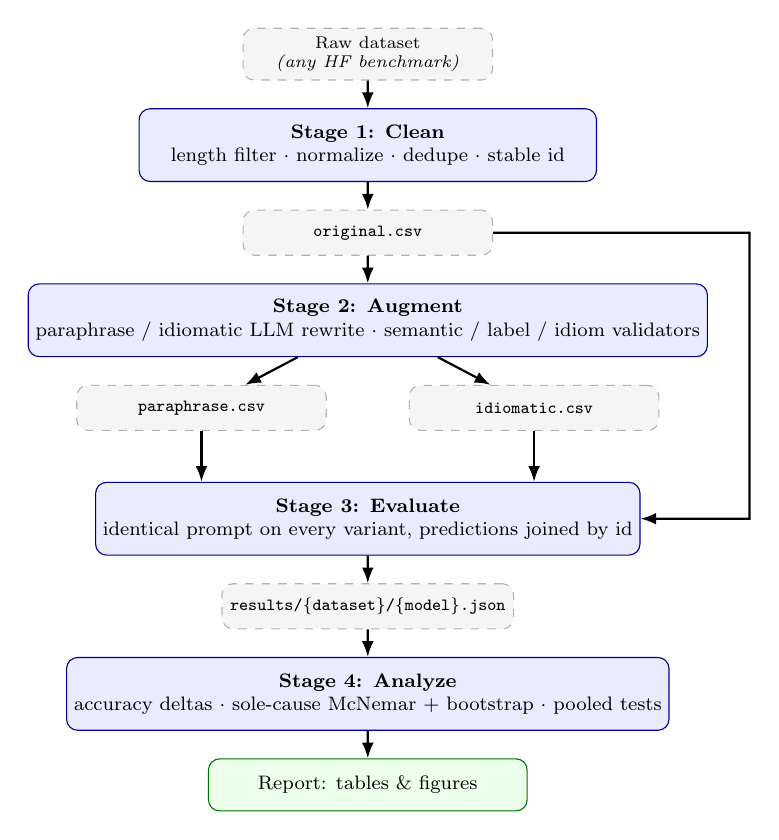
\begin{tikzpicture}[
    scale=0.88, every node/.style={transform shape},
    node distance=4mm and 5mm,
    stage/.style={rectangle, rounded corners, draw=blue!60!black, fill=blue!8,
      minimum width=6.6cm, minimum height=1.05cm, align=center, font=\footnotesize, inner sep=3pt},
    artifact/.style={rectangle, rounded corners, draw=gray!60, fill=gray!8, dashed,
      minimum width=3.6cm, minimum height=0.65cm, align=center, font=\scriptsize},
    finalbox/.style={rectangle, rounded corners, draw=green!45!black, fill=green!8,
      minimum width=4.6cm, minimum height=0.75cm, align=center, font=\footnotesize},
    arrow/.style={-{Latex[length=2mm]}, thick}
  ]
  \node[artifact]                (raw)  {Raw dataset\\ \textit{(any HF benchmark)}};
  \node[stage, below=of raw]     (s1)   {\textbf{Stage 1: Clean}\\ length filter $\cdot$ normalize $\cdot$ dedupe $\cdot$ stable id};
  \node[artifact, below=of s1]   (orig) {\texttt{original.csv}};
  \node[stage, below=of orig]    (s2)   {\textbf{Stage 2: Augment}\\ paraphrase / idiomatic LLM rewrite $\cdot$ semantic / label / idiom validators};
  \node[artifact, below=of s2, xshift=-2.4cm] (para) {\texttt{paraphrase.csv}};
  \node[artifact, below=of s2, xshift=2.4cm]  (idio) {\texttt{idiomatic.csv}};
  \node[stage, below=18mm of s2] (s3)   {\textbf{Stage 3: Evaluate}\\ identical prompt on every variant, predictions joined by id};
  \node[artifact, below=of s3]   (res)  {\texttt{results/\{dataset\}/\{model\}.json}};
  \node[stage, below=of res]     (s4)   {\textbf{Stage 4: Analyze}\\ accuracy deltas $\cdot$ sole-cause McNemar + bootstrap $\cdot$ pooled tests};
  \node[finalbox, below=of s4]   (rep)  {Report: tables \& figures};

  \draw[arrow] (raw)  -- (s1);
  \draw[arrow] (s1)   -- (orig);
  \draw[arrow] (orig) -- (s2);
  \draw[arrow] (s2)   -- (para);
  \draw[arrow] (s2)   -- (idio);
  % variants drop straight down onto the top edge of Stage 3
  \draw[arrow] (para.south) -- (para.south |- s3.north);
  \draw[arrow] (idio.south) -- (idio.south |- s3.north);
  % original.csv bypasses Stage 2 down the right-hand side and enters Stage 3
  % at its east edge; the bypass column sits clear of every box to its left
  % bypass column: x taken from s2.east (the widest box, since its text exceeds
  % the minimum width), y taken from orig so the first leg stays horizontal
  \coordinate (bypassx) at ($(s2.east)+(0.6,0)$);
  \coordinate (bypass)  at (bypassx |- orig.east);
  \draw[arrow] (orig.east) -- (bypass) -- (bypass |- s3) -- (s3.east);
  \draw[arrow] (s3)   -- (res);
  \draw[arrow] (res)  -- (s4);
  \draw[arrow] (s4)   -- (rep);
\end{tikzpicture}
\caption{The four-stage pipeline (dataset- and model-agnostic; the same
pipeline instantiates once per dataset/model combination). Raw data is
cleaned (Stage 1), rewritten into validated paraphrase and idiomatic
variants (Stage 2), evaluated per model across every variant with an
identical prompt (Stage 3), and aggregated into the accuracy-delta and
sole-cause significance analysis (Stage 4). \texttt{original.csv} feeds both
Stage 2 (as the rewriting source) and Stage 3 (as the control variant)
directly.}
\label{fig:pipeline}
\end{figure}

\textbf{Stage 1: Clean.} Each raw dataset is loaded from Hugging Face and
reduced to a single clean CSV of rows suitable for rewriting: rows whose
input length (in whitespace-delimited tokens) falls outside a configured
band are dropped (very short inputs leave no room for an idiom to be
inserted naturally; very long inputs are expensive to augment and dilute the
measured effect), text is normalized (Unicode NFC, whitespace collapsing),
exact duplicates are removed, and every retained row is assigned a stable
identifier used to align all downstream variants of that row. The label $y$
and any dataset-specific metadata (e.g. MMLU's answer choices) are carried
through unchanged.

\subsection{Augmentation into paraphrase and idiomatic variants}
\label{sec:augmentation}

\textbf{Stage 2: Augment.} Each cleaned row is rewritten by an external
LLM (Google Gemini, selected via config; Anthropic Claude and OpenAI GPT are
also supported behind the same client interface) into two variants using two
distinct, fixed prompt templates. Templates are selected per dataset, so a
task whose input is not a free-standing sentence can use wording suited to it
(MNLI, whose rewrite target is a premise judged against a fixed hypothesis,
uses its own NLI-specific pair of templates) without perturbing the prompt
hashes, and therefore the warm caches, of the other datasets:

\begin{itemize}
  \item \emph{Paraphrase prompt}: instructs the augmenter to reword the
    text in different words while explicitly avoiding idiomatic expressions,
    preserving meaning.
  \item \emph{Idiomatic prompt}: instructs the augmenter to reword the
    text so that it naturally incorporates one or more idiomatic
    expressions or figures of speech, while preserving meaning, register,
    and length, and explicitly preserving the task label $y$ (the label is
    passed into the prompt itself so the rewrite cannot silently invert the
    correct answer, e.g. flipping a positive sentiment snippet into a
    negative one).
\end{itemize}

An external, deliberately stronger LLM is used for augmentation rather than
one of the models under evaluation, since the augmenter's own idiom/paraphrase
judgment needs to be more reliable than the systems being tested. Every
augmented row is passed through a validator chain before being accepted:

\begin{itemize}
  \item \textbf{Semantic similarity} to the original text, above a fixed
    cosine-similarity threshold.
  \item \textbf{Label preservation}: an LLM-judge check that the rewrite
    has not altered the correct task label.
  \item \textbf{Idiom presence / absence}: an LLM-judge check specific to
    each variant; the idiomatic variant must contain a genuine idiomatic
    expression, and the paraphrase variant must \emph{not}.
\end{itemize}

Rows that fail validation after a bounded number of retries are dropped from
that variant (recorded in a sidecar manifest for transparency), which is why
the paraphrase/idiomatic CSVs are typically somewhat smaller than the
original CSV. An on-disk response cache, keyed by (prompt hash, augmenter
model, input id), makes reruns idempotent and avoids re-incurring API cost
for rows that have already been successfully augmented under an unchanged
configuration.

\subsection{Datasets}

\begin{itemize}
  \item \textbf{SST-2} \citepf{socher2013sst}: binary sentiment
    classification over short movie-review snippets, in the GLUE split
    \citepf{wang2019glue}; metric: accuracy.
  \item \textbf{MMLU} \citepf{hendrycks2021mmlu}: multiple-choice
    multi-domain knowledge questions spanning 57 subjects; metric: accuracy.
  \item \textbf{MNLI (MultiNLI)} \citepf{williams2018mnli}: three-way natural
    language inference (\emph{entailment} / \emph{neutral} /
    \emph{contradiction}) over premise--hypothesis pairs drawn from ten
    written and spoken genres; metric: accuracy.
\end{itemize}

These three datasets were chosen to cover qualitatively different task types
under the same paraphrase/idiom protocol: short, informal,
already-somewhat-figurative text (SST-2 movie-review snippets); longer,
formal, fact-oriented multiple-choice questions (MMLU); and sentence-pair
inference (MNLI), to see whether an idiom-degradation effect (if present)
generalizes across task style. MNLI is the most direct test of the three: in
sentiment classification or knowledge QA an idiom perturbs the surface form
of an input whose answer is otherwise independent of it, whereas an
entailment judgement turns on a literal reading of the premise itself, so
idiomatic phrasing bears on the decision rather than merely on its wording.
Its three-way label space also sets chance at 33\% rather than 50\%, which
depresses the per-row rate of sole-cause events relative to a binary task.

\textbf{MNLI-specific protocol.} Two aspects of the MNLI instantiation differ
from the other two datasets and are worth stating explicitly, since both bear
on the validity of the paired analysis in \S\ref{sec:stats}:

\begin{itemize}
  \item \textbf{Only the premise is rewritten.} The hypothesis is carried
    through in metadata and stays byte-identical across the original,
    paraphrase, and idiomatic variants, so the manipulation is confined to one
    side of the pair and cannot alter the hypothesis it is judged against.
  \item \textbf{One row per premise.} MNLI pairs roughly three hypotheses with
    every premise; emitting all of them would place the same premise in the
    dataset several times, violating the independence assumption underlying
    the paired test. The loader therefore keeps only the first hypothesis per
    premise.
\end{itemize}

Rows are drawn from the two validation splits combined (matched, 9{,}815
pairs; mismatched, 9{,}832), rather than from the training split, and the
test split is unusable here because its labels are withheld. Because the
mismatched half contributes the five genres absent from training, each row's
genre is recorded alongside it so that genre shift remains visible as a
potential confound rather than being silently absorbed into the comparison.
After first-hypothesis selection and cleaning, 5{,}127 premises survive to
form the MNLI \texttt{original.csv}.

\subsection{Evaluated models}

Rather than a single-model case study, this project evaluates a broad panel
of eleven open, instruction-tuned decoder LLMs spanning roughly 0.5B to 9B
parameters across several distinct model families and pretraining lineages:
the Qwen2.5-Instruct family (0.5B / 1.5B / 3B / 7B), the Gemma-2-it family
(2B / 9B), Mistral-7B-Instruct-v0.3, Phi-4-mini-instruct,
DeepSeek-R1-Distill-Qwen-7B, SmolLM2-1.7B-Instruct, and
StableLM-2-1.6B-Chat. Deliberately spanning multiple parameter scales
\emph{within} the same family (e.g. four Qwen2.5 sizes) as well as multiple
\emph{different} families at similar scale lets the analysis separate
size-driven effects from family/architecture-driven effects, rather than
conflating the two, as a single model or a single family swept across sizes
would. All models are evaluated zero-shot, with an identical dataset-specific
prompt template applied to all three variants of a given row so that only
the input text differs between runs; a single device-agnostic runner
transparently selects CUDA, Apple-Silicon MPS, or CPU execution and adjusts
precision accordingly.

\textbf{Stage 3: Evaluate.} For each (model, dataset) pair, the model is
run on all three variant CSVs with the identical prompt, and predictions are
joined by row id, yielding one matched (original, paraphrase, idiomatic)
triple of predictions per surviving row. Per-variant accuracy is computed
directly from these joined predictions.

\subsection{Statistical framework}
\label{sec:stats}

\textbf{Stage 4: Analyze.} Beyond simple per-variant accuracy and its
paraphrase/idiom deltas, the primary diagnostic used in this project is a
\emph{sole-cause} test, designed specifically to attribute degradation to a
single rewrite type rather than to ordinary noise:

\begin{enumerate}
  \item Restrict to rows where all three variants were successfully
    produced and where the model answered the \textbf{original} variant
    correctly (so any subsequent error is attributable to the rewrite, not
    to the task itself being hard for that model).
  \item For each such row, record the joint correctness outcome across the
    paraphrase and idiomatic variants: one of four combinations (both
    correct, both incorrect, paraphrase-only-incorrect, idiomatic-only-
    incorrect).
  \item Count $b$ = \emph{idiomatic-only-wrong} (idiomatic rewrite alone
    broke an otherwise-correct answer) and $c$ = \emph{paraphrase-only-
    wrong} (paraphrase rewrite alone broke it). Rows where both rewrites
    agree (both broke it, or neither did) carry no information about which
    rewrite is worse and are excluded, exactly as in any paired test.
\end{enumerate}

The significance of the gap between $b$ and $c$ is assessed two ways:

\textbf{McNemar's test} \citepf{mcnemar1947note}, with the continuity
correction of \citetf{edwards1948note}:
\begin{equation}
  \chi^2 = \frac{(|b - c| - 1)^2}{b + c}, \qquad \mathrm{df} = 1,
\end{equation}
testing the null hypothesis that $b$ and $c$ are drawn from the same
underlying 50/50 rate (i.e. among discordant rows, it is a coin flip which
rewrite broke it).

\textbf{Non-parametric bootstrap check.} Because McNemar's test relies on a
chi-square approximation that can be unreliable when $b + c$ is small, every
result is cross-checked with a paired bootstrap
\citepf{efron1993bootstrap,koehn2004significance}:
the aligned rows are resampled with replacement 10{,}000 times, the
difference $b - c$ is recomputed on each resample, and a 95\% percentile
confidence interval plus a two-sided empirical p-value are read off the
resulting empirical distribution. A result is only treated as robustly
significant when both the classical and the non-parametric check agree;
when they disagree, the more conservative (non-significant) verdict is
preferred.

The same sole-cause statistics are additionally pooled across all evaluated
models for a given dataset (summing $b$ and $c$, and resampling from the
concatenated pooled rows for the bootstrap), with the explicit caveat that
this pooling is not a rigorous mixed-effects test, since different models
are not strictly exchangeable independent draws, and is reported as
indicative rather than definitive.

\section{Experimental results}

\textit{[To be completed once the full evaluation sweep and statistical
analysis are finalized.]}

\section{Discussion}

\textit{[To be completed alongside the experimental results above.]}

\section{Code}

Code repository: \url{https://github.com/LihuZur/Idiom_degredation} % TODO: confirm final repo URL/visibility before submission

\bibliographystyle{unsrtnat}
\bibliography{references}
\end{document}
